\section{The Gauss-Bonnet Theorem}



The Gauss-Bonnet theorem for regular surfaces states

\begin{theorem}[The Continuous Gauss-Bonnet Theorem] \label{thm:g-b-c}

If $M$ is a regular surface with boundary $\partial M$ then
	$$\int_{M} K dA+ \int_{\partial M} k_g ds + \sum_i \beta_i= 2\pi \chi(M)$$
	where  $K$ is Gaussian curvature,
	 $k_g$ is the geodesic curvature,
	 each $\beta_i$  is an exterior angle at a vertex of the boundary and
	$\chi$ is the Euler characteristic.
\end{theorem}


The  Gauss-Bonnet theorem is  telling us, if we add up curvature
at each vertex the sum will be $2\pi$ times to Euler characteristic.
The curvature at each vertex is computed by considering a 'local' neighborhood
around the vertex and we learn global topological information. Thus, the Gauss-Bonnet 
theorem is an example of a local to global principle. 
Conversely, if we know the Euler characteristic we can learn about the curvature
at individual points. We will often use the theorem to prove the existence of
a vertex with a desirable amount of curvature.



\subsection{Banchoff's Proof}
We now include a proof of a combinatorial version of the theorem due to Banchoff
\cite{banchoff_critical_1970}. We will first use another local to global theorem,
the Critical Point theorem, which we now define.
Given a regular surface embedded in $\R^3$ consider a line $\ell$ and define a linear height function $h:M \to \R$
to be the projection of all of $\R^3$ on to the line $\ell$. A point $p$ on $M$
is a \emph{critical point} for $\ell$ if the tangent plane at $p$ is perpendicular to $\ell$.
All points on $M$ that are not critical are \emph{ordinary point}.
Critical points can be classified into three categories, maxima, minima, and saddle points.
We define the \emph{index} of a critical point, denoted $i(p,h)$, to be 
$i(p,h)=1$ if $p$ is a  local maximum or minimum and $i(p,h)=-1$ is $p$ is a saddle point.
An example is shown in \figref{torus-total}.
The \emph{Critical  Point theorem} states that if the number of critical points is finite
then 
\begin{equation} \label{eqn:critical-point-theorem}
	\sum_{p\ \textrm{critical}} i(p,h)=\chi(M).
\end{equation}


 \begin{figure}[htb]
         \centering
        \begin{subfigure}[b]{0.3\textwidth}
         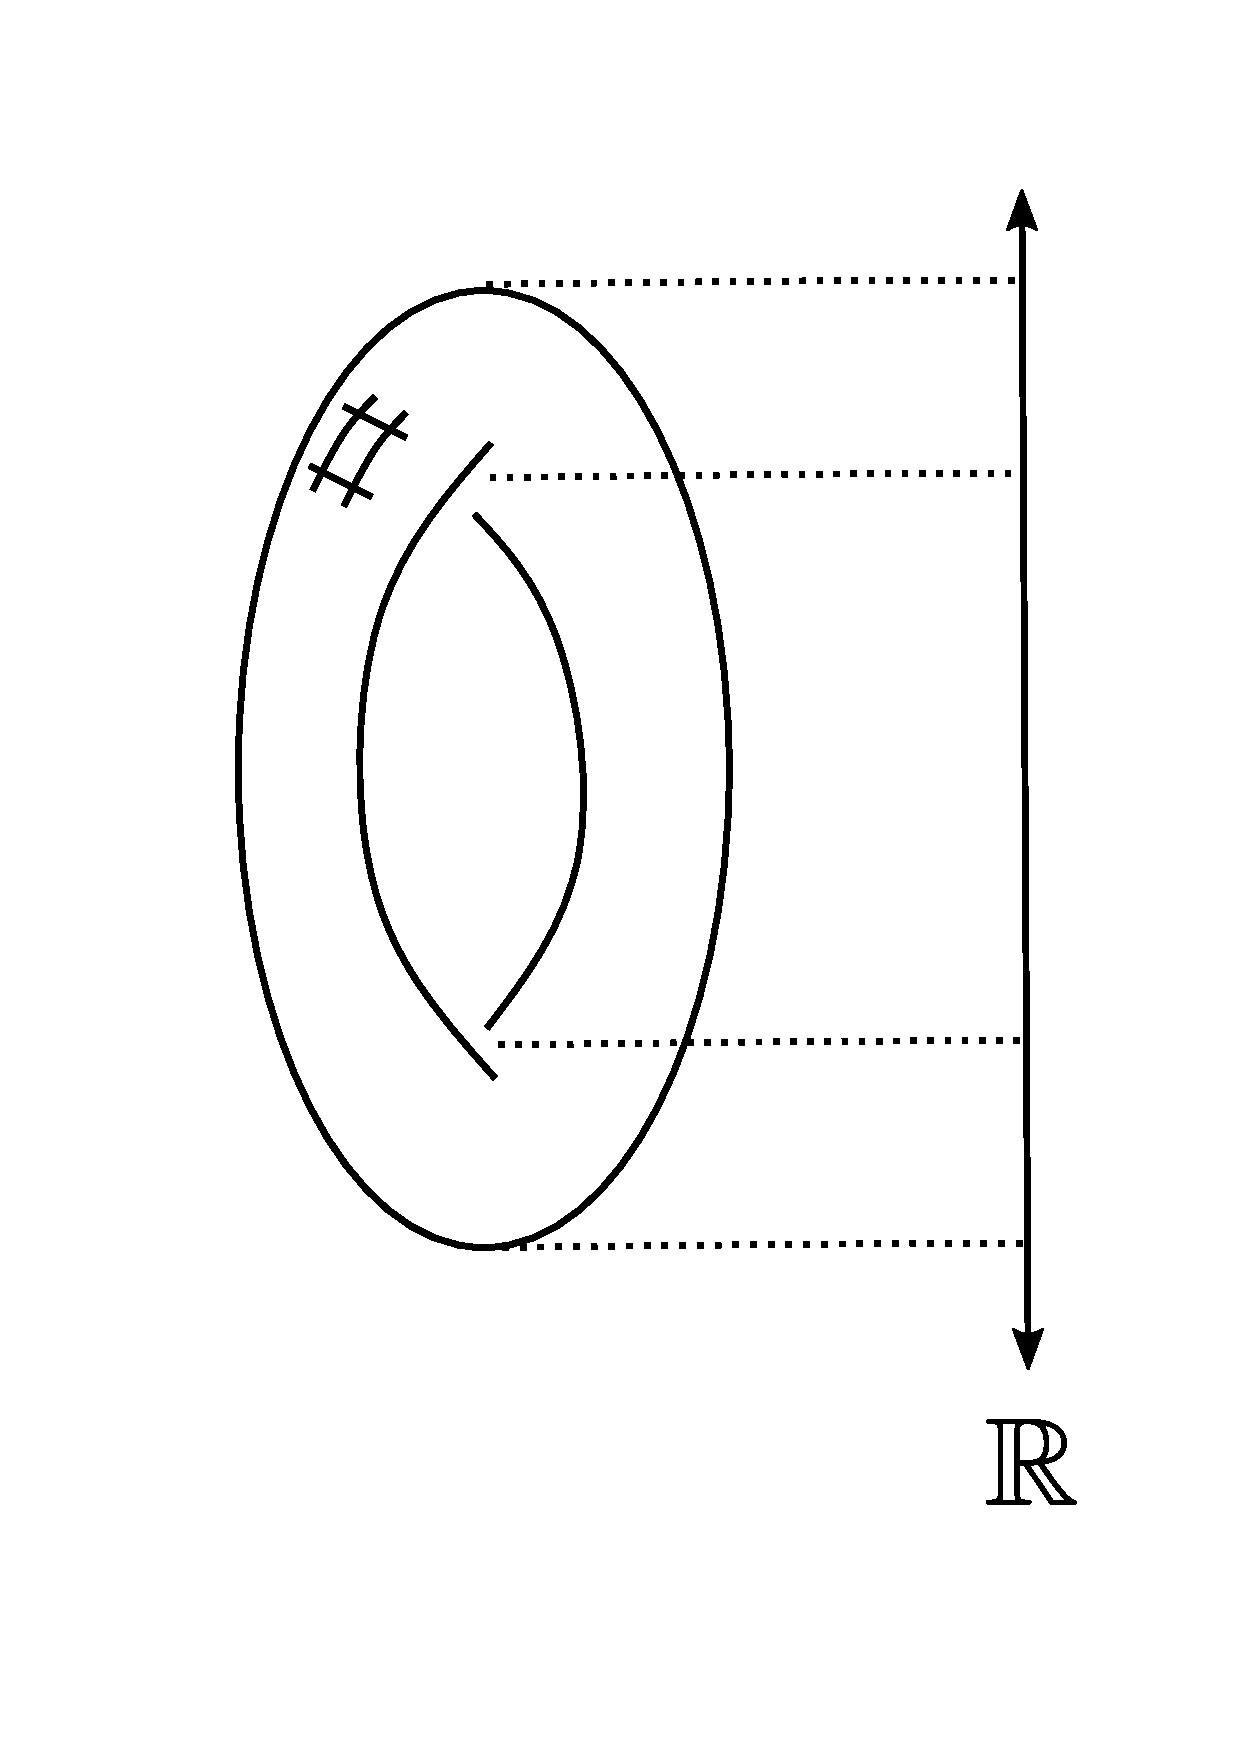
\includegraphics[width=\textwidth]{chapter-3/torus}
         \subcaption{The tours a line $\ell$ with four critical points.}
 	 \label{fig:torus-ell}
       \end{subfigure}\\
         \begin{subfigure}[b]{0.21\textwidth}
         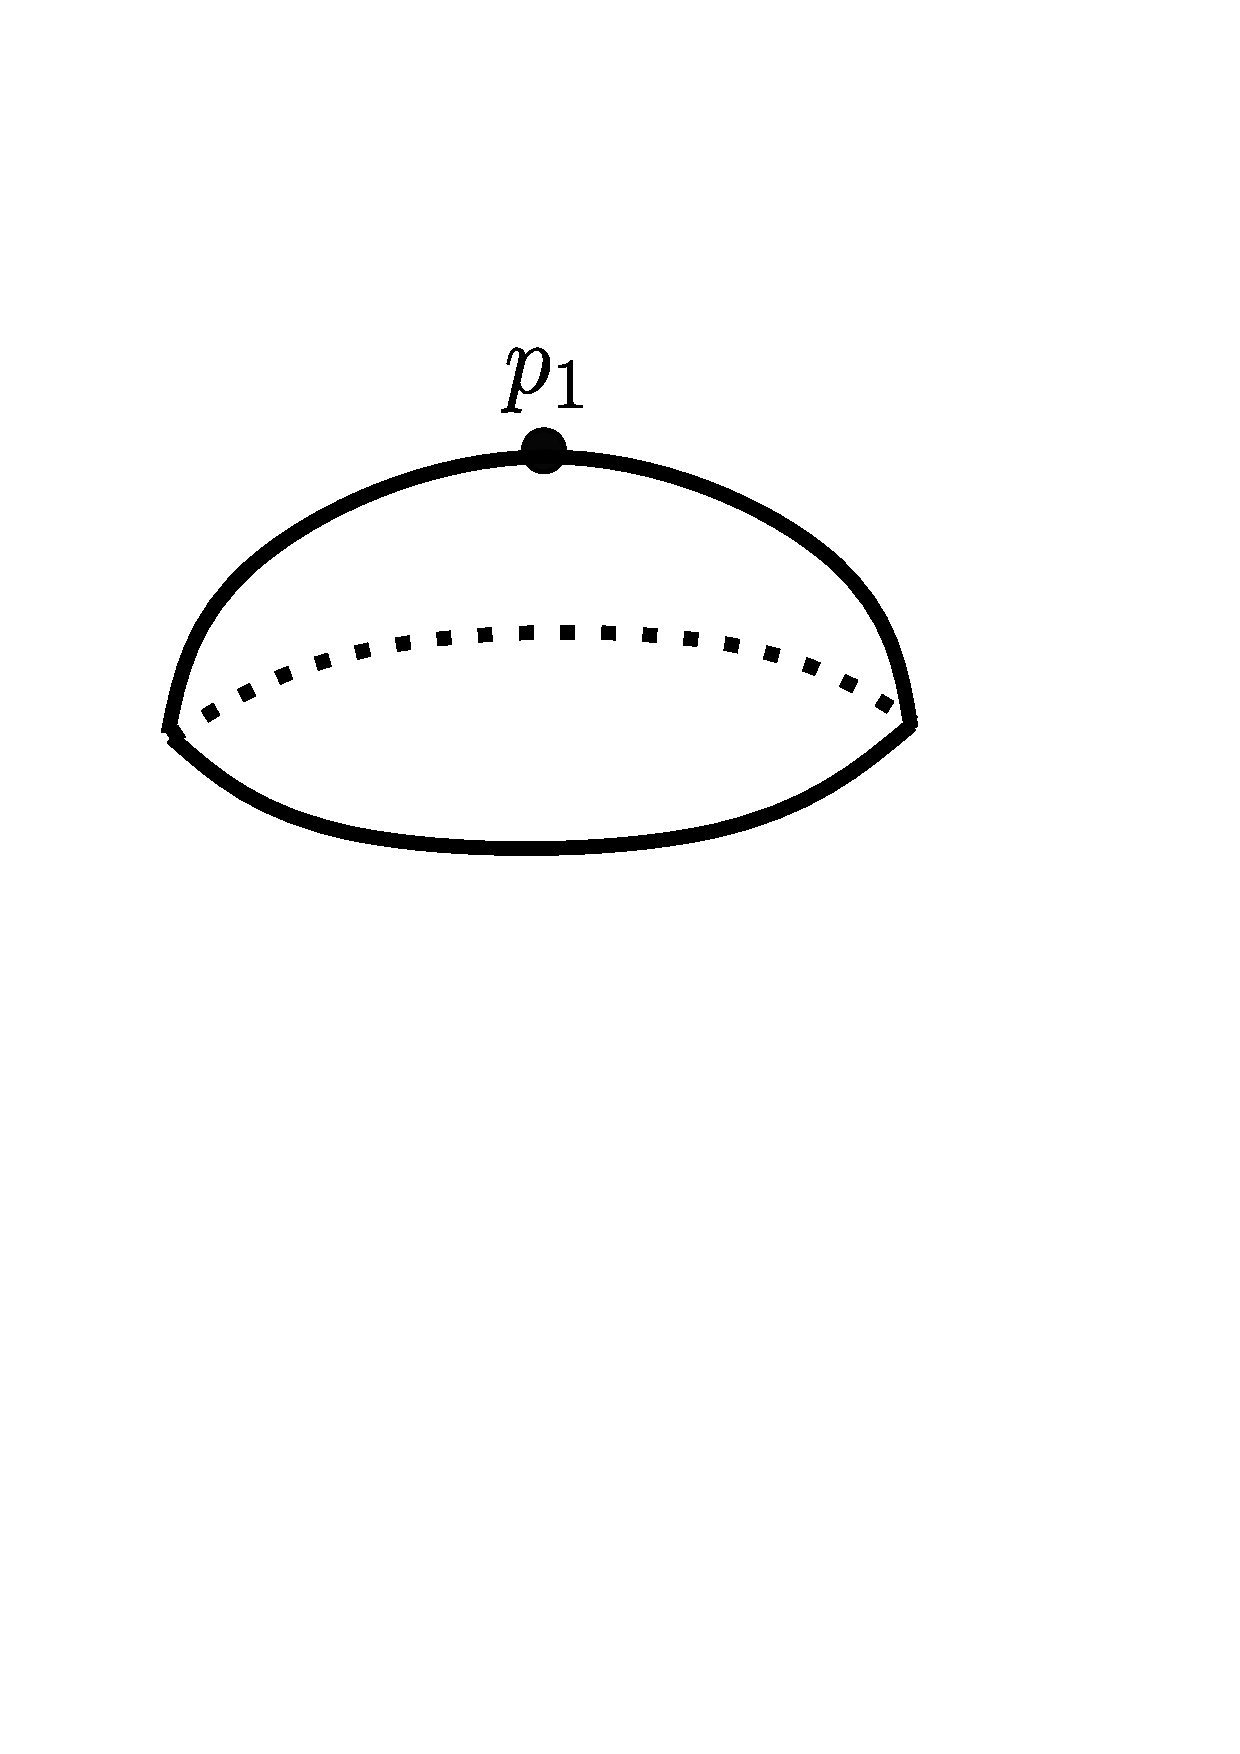
\includegraphics[width=\textwidth]{chapter-3/torus-top}
         \subcaption{Local to $p_1$.}
          \label{fig:max}
         \end{subfigure}
          \begin{subfigure}[b]{0.21\textwidth}
         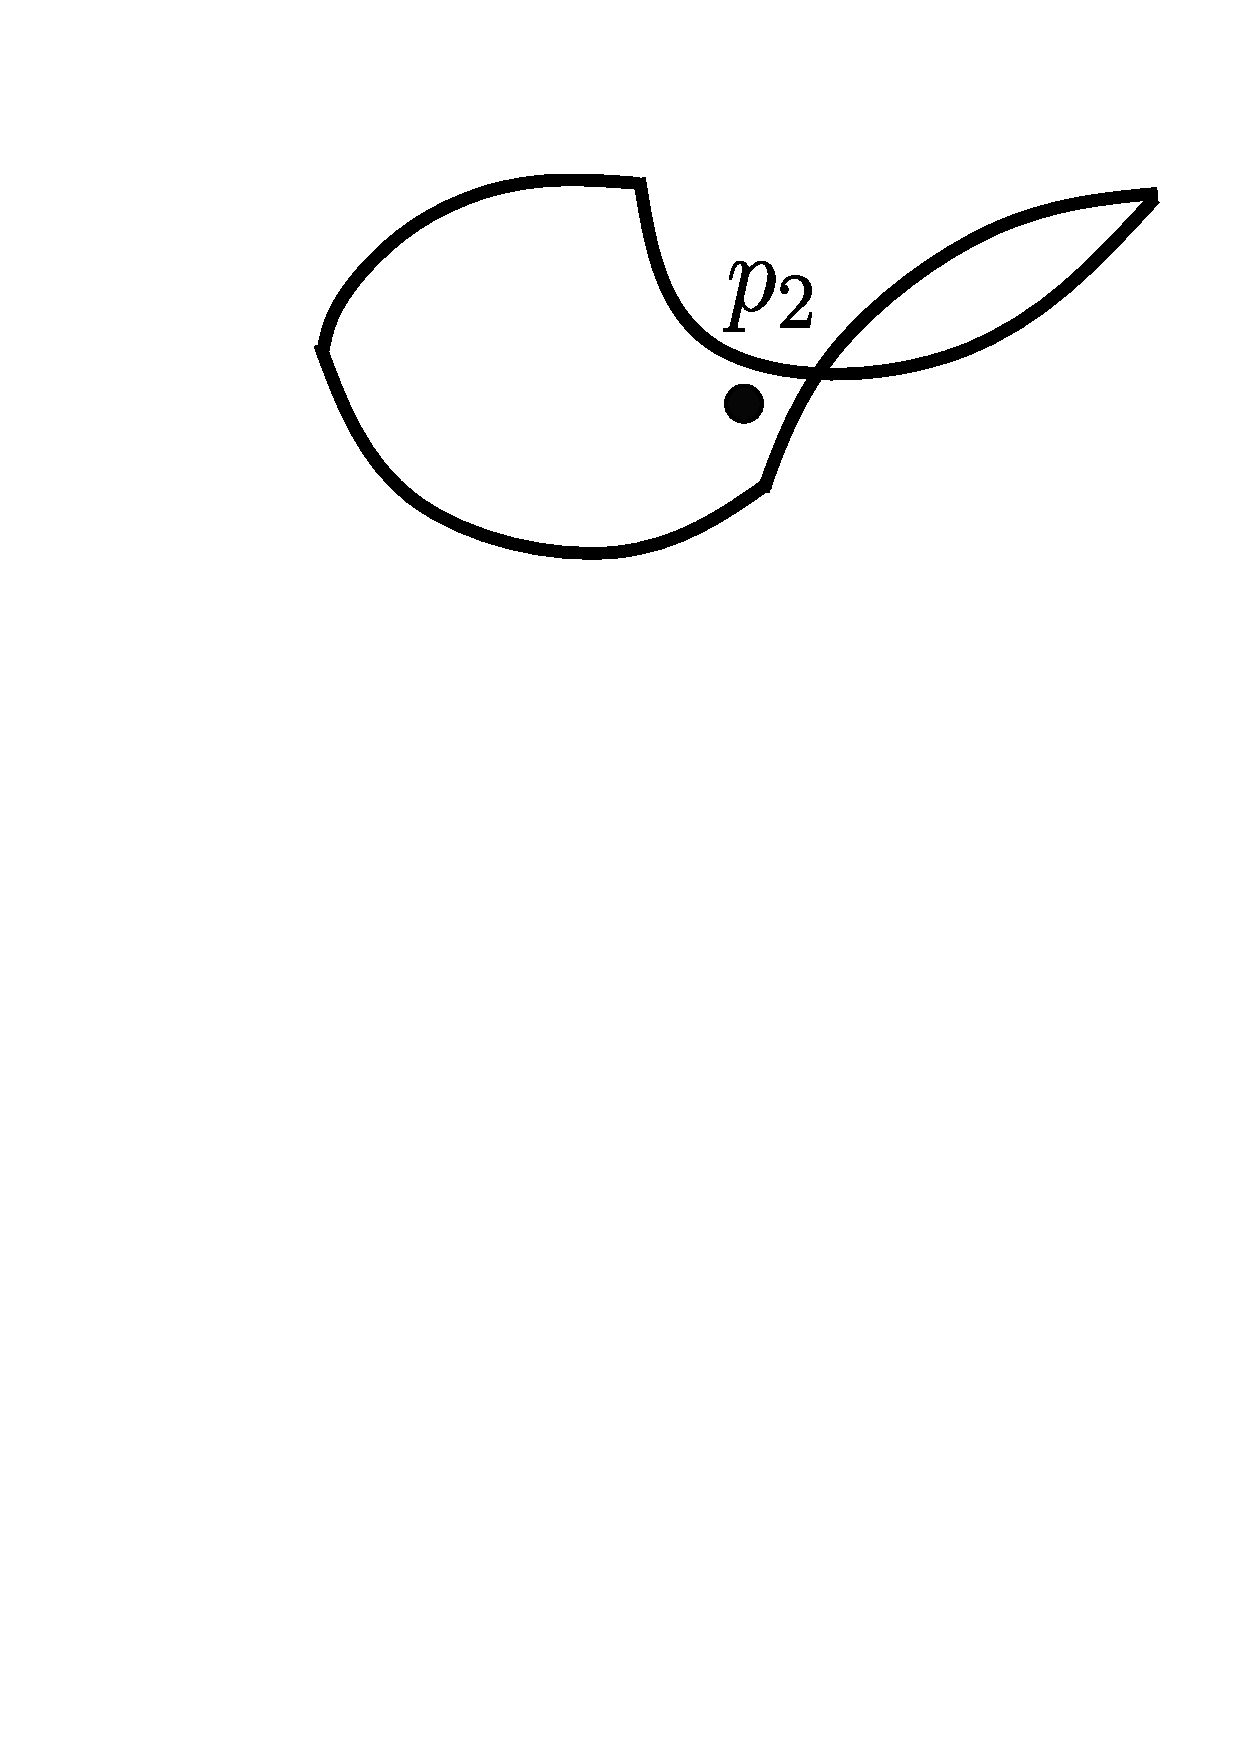
\includegraphics[width=\textwidth]{chapter-3/saddle1}
         \subcaption{Local to $p_2$.}
          \label{fig:saddle1}
         \end{subfigure}
         \begin{subfigure}[b]{0.21\textwidth}
         \includegraphics[width=\textwidth]{chapter-3/saddle2}
         \subcaption{Local to $p_3$.}
          \label{fig:saddle2}
         \end{subfigure}
         \begin{subfigure}[b]{0.21\textwidth}
         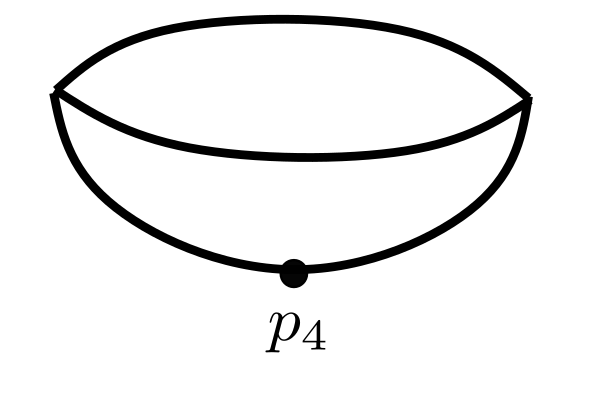
\includegraphics[width=\textwidth]{chapter-3/torus-bottom}
         \subcaption{Local to $p_4$.}\label{fig:min}
         \end{subfigure}
		\caption{(\subref{fig:torus-ell}) A tours and line $\ell$. There are four critical points.
 		(\subref{fig:max}) The critical point $p_1$ is a maximum and $i(p_1,h)=1$.
		(\subref{fig:saddle1}) The critical point $p_2$ is a saddle and $i(p_1,h)=-1$.
		(\subref{fig:saddle2}) The critical point $p_3$ is also a saddle and $i(p_1,h)=-1$.
		(\subref{fig:min}) The critical point $p_4$ is a minimum and $i(p_1,h)=1$.
 		\label{fig:torus-total}}
 \end{figure}








